\documentclass[review]{elsarticle}
%-----------------------------------------------------

\usepackage{amsmath}
\usepackage{graphicx}

\graphicspath{{./figs/}}

\newcommand{\ihat}{\boldsymbol{\hat{\textbf{\i}}}}
\newcommand{\jhat}{\boldsymbol{\hat{\textbf{\j}}}}
\newcommand{\roughly}{{\raise.17ex\hbox{$\scriptstyle\sim$}}}
\newcommand{\dmax}{d_\text{max}}
\newcommand{\dmin}{d_\text{min}}

%-----------------------------------------------------

\makeatletter
\renewcommand{\fnum@figure}{Figure 8}
\makeatother

\thispagestyle{empty}

\begin{document}
\allowdisplaybreaks

\begin{figure}[ht]
\centering
%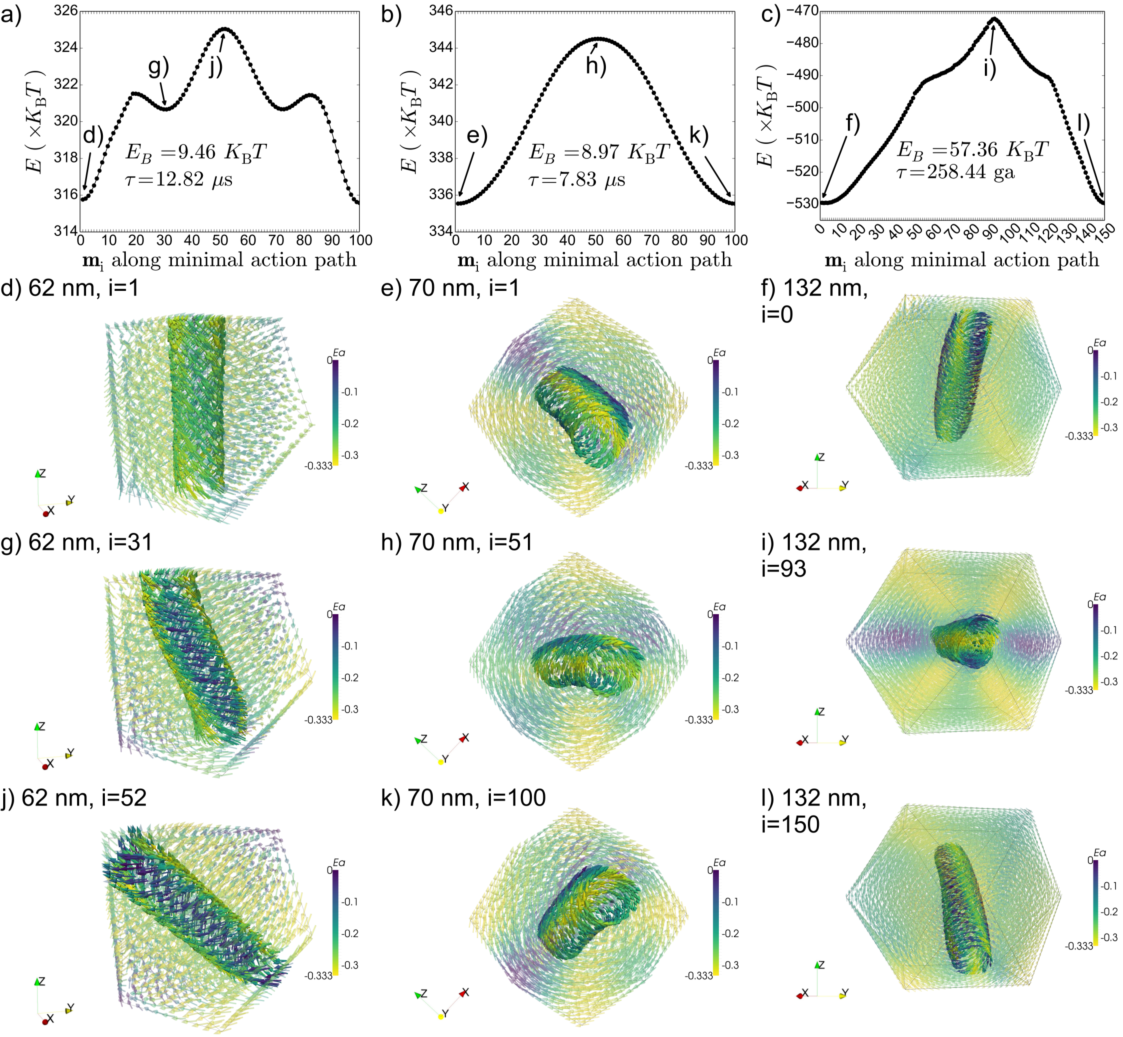
\includegraphics[width=\textwidth]{Figure_08_HR.pdf}
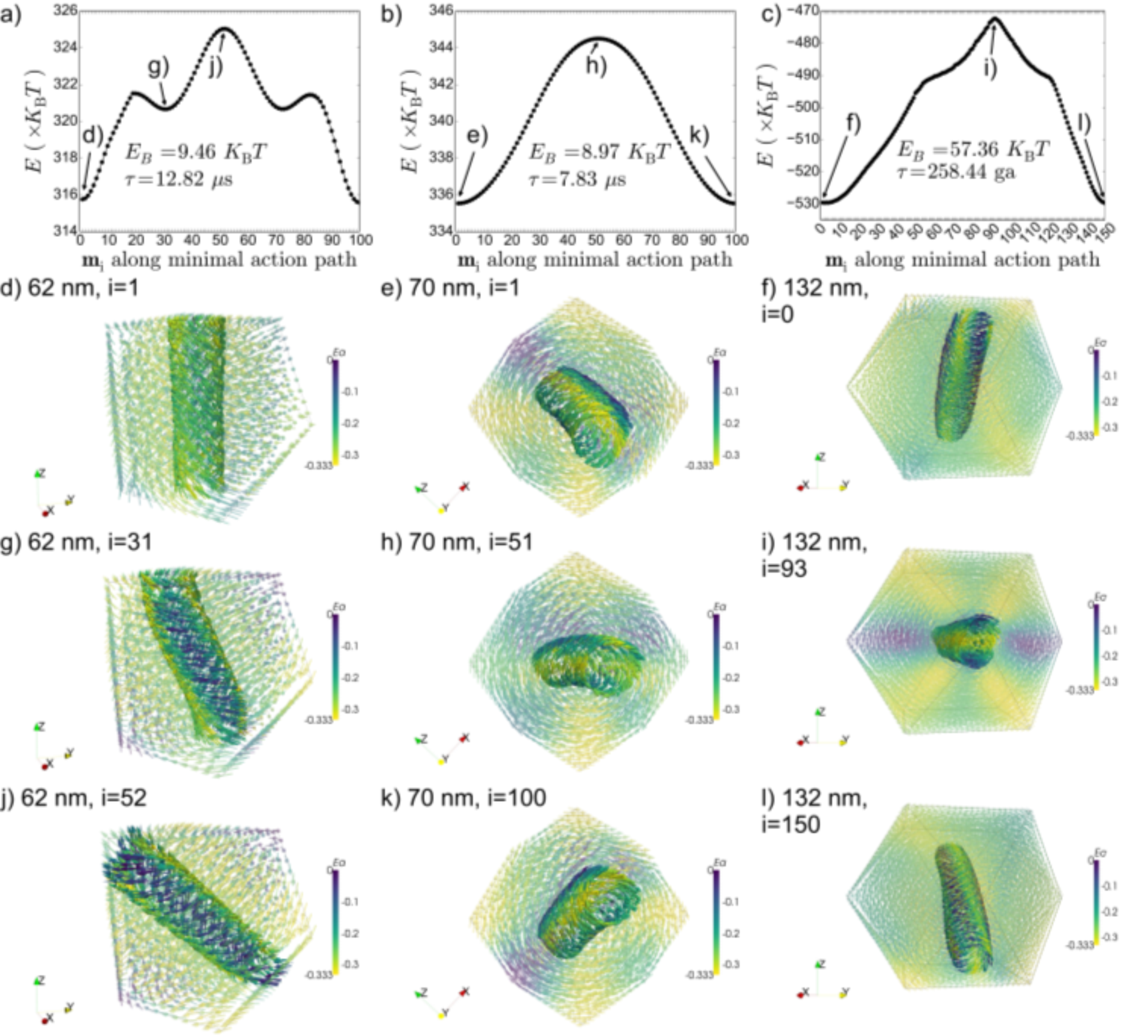
\includegraphics[width=\textwidth]{Figure_08.pdf}
\caption{Action-minimising paths for the cuboctahedra. The cuboctahedra showed different AMPs above the SD--PSD threshold from the rest of the shapes. Above the SD--PSD threshold, and up to 66$\,\text{nm}$, the lowest energy state for the cuboctahedron is a HAV. Transitions between HAVs (left column) occur via a distortion (g) and structured rotation (j) of the vortex core. The energy barrier is an IAV (j). The dIAV along the AMP (g) sits in its own LEM, forming a three-bump energy barrier (a). The dIAV becomes the lowest energy from 66$\,\text{nm}$. Transitions between dIAVs (center column) form a single bump energy barrier (b). The transition is a structured rotation of the distorted vortex, keeping attached to the same surface (e, h, k). Once the lowest energy is an EAV, transitions between these (right column) occur via a distortion and structured rotation of the vortex core. The energy barrier is an IAV (i). Colour represents the MCA energy normalised by $|K_1|$. The energies along the AMPs are plotted in units of $K_\text{B}T$, with $T=300\,\text{K}$. The right column of Video 1 (supplementary material) shows these transitions.}
\label{fig8}
\end{figure}

\end{document}